\section{Introduction}
\label{sec:intro}


\section{Background}
\label{sec:background}

\subsection{RDMA}

RDMA is a networking technology which allows client machines
to directly access the memory of a remote server. RDMA is an
enabling technology for memory disaggregation as
\textit{memory servers} do not need any computation
resources (save setting up the RDMA memory initially).

One sided RDMA verbs (read, write, atomic) are used to
access remote memory without any memory side computation.
One sided verbs require RDMA reliable connections which
guarantee in-order delivery of operations.


\subsection{Remote Memory Data Structures}

\section{Problems}
\label{sec:problems}

Designing data structures for remote memory is hard. The
primary reason is that there is no centralized serialization
point to guard access to remote memory. Traditional key
value stores (Memcached~\cite{memcached}), and even RDMA
based Key-value stores~\cite{herd,erpc,pilaf} use a mixture
of one-sided and two-sided verbs. Normally writes are two
sided, and the memory-side CPU performs locking close to
memory and ensures that all writes are issued in order.

In remote memory, no such CPU exists. To get serialization
expensive RDMA atomic operations like \textit{compare and
swap}(CAS) must be used. Atomic operations are by no means a
silver bullet. With a CPU close to memory critical sections
are small. Consider inserts into a cuckoo hash table with a
long path. The CPU acquires some number of locks in memory
then performs a series of reads and wites to commit the path
before unlocking. Reads writes and locking only consumes a
memory access ~50ns which keeps the critical section small.
In contrast locking with RDMA atomic operations and
performing multiple lookups is very expensive.

First, acquiring a lock means a round trip. If the table has
a single lock, then a client is guaranteed to be able to
gather all the locks it requires in a single round trip.
However a single lock does not scale as only a single writer
can write at a time. This matter is made worse by the fact
that the critical section of the lock is larger in remote
memory. Breaking the table up into subtables each with it's
own lock has it's own problems. An insertion with a long
path will potentially need to acquire many locks. Each of
which requires a round trip. Therefore using fine grained
locking increases the tables scalability but increases it's
base case insertion time.

\textbf{Read Optimization} Most data center workloads are
read heavy, therefore read operations should be the most
highly optimized~\cite{datacenter-workloads}. Prior
approaches such as RACE require two RDMA round trips per
read. The first is a hash index lookup, the second round
trip reads the actual key-value block. RACE must perform two
round trips because entries in the hash index are limited to
64 bits (CAS width). This is commonly not enough to store
both key and value so RACE can not inline both keys and
values in the index structure. Clover~\cite{clover} enables
single round trips reads. However under contention Clovers
reads require pointer chasing which is known to be expensive
due to each pointer resolution requiring a round
trip~\cite{clio,clover,pointer-chaising}. Ideally we would
be able to ensure that reads complete in a single round
trip.


\section{Design}
\label{sec:design}

\subsection{Locality Hashing}
\begin{figure*}[t]
    \centering
    \begin{subfigure}{0.3\linewidth}
        \begin{align*}
            L_1 &= h_1(k) \\
            L_2 &= L_1 + h_2(k) \% f^{f + log_2(h_3(k))}
        \end{align*}
        % \caption{}
        \label{fig:hash_factor}
    \end{subfigure}
    \begin{subfigure}{0.3\linewidth}
        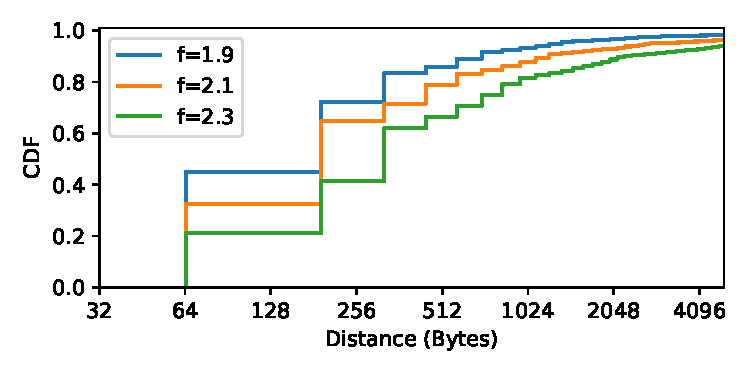
\includegraphics[width=0.99\linewidth]{fig/hash_factor.pdf}
        \label{fig:hash_factor}
        % \caption{}
    \end{subfigure}
    \begin{subfigure}{0.3\linewidth}
        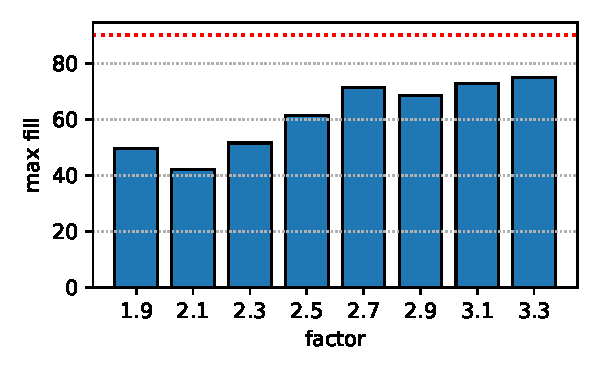
\includegraphics[width=0.99\linewidth]{fig/hash_fill.pdf}
        \label{fig:hash_fill}
        % \caption{}
    \end{subfigure}.
    \vspace{-1em}
    \caption{
    \textbf{(a)} Dependent hashing for factor $f$.
    \textbf{(b)} CDF of distances between cuckoo locations dependent hashing on different exponential factors.
    \textbf{(c)} Exponential factor relation to max fill in cuckoo hash.
    }
    \label{fig:locality-hashing}

\end{figure*}

Cuckoo hashing and Hopscotch hashing are both read optimized
hash tables. Cuckoo hashing ensures that all reads are at
most two memory accesses~\cite{cuckoo}, while hopscotch
hashing ensures that a read is within a bounded range of
it's hash index~\cite{hopscotch}. Both of these properties
have been noticed by the RDMA key-value store, and far
memory communities for their fast
reads~\cite{memc3,cuckoo-improvements,pilaf,farm}.

Our approach aims to combine the bounded reads of cuckoo
hashing, with the locality properties of hopscotch hashing.
To do so we bound the distance between cuckoo hash
locations. Traditional cuckoo hashing calls for two
independent hash functions. We instead make our two hash
functions dependent. The first hash function determines the
location a key will be hashed to. The second hash function
determines the maximum distance the second value can have
from the first. A third hash function determines a random
location between the first location, and the bound imposed by
the second.

A strawman implementation of locality based hashing would
use the first hash function to find a location, and the
second to find a random location within a fixed bound. This
approach quickly leads to failed insertions. Due to the
birthday paradox the probability of a collision is high, and
on large tables the probability that one region of the hash
table will become full, and have not viable path to an open
slot is high. ~\todo{Insert a figure of one of my failed
insertion experiments on a big table}.

Rather than use a static bound we use a dynamic logarithmic
bound. The bound set by the second hash function is
determine by counting the suffix zeros of the resultant hash
and rasing it by an exponential factor. In the common case
the bound is small, but on an exponentially decrease rate
some pairs of values are spaced far apart. This design
enables some pairs to act as ~\textit{waypoints} to other
regions of the table. This method, paired with associative
in the cuckoo hash enables high fill rates while keeping the
region of the table any given key can inhabit
small.

Figure~\ref{fig:locality-hashing} illustrates the tradeoff
between locality and maximum fill factor. 

\subsection{Locking}

Traditional wisdom would suggest that because cuckoo hashing
can have long insertion paths it is a poor candidate for
remote memory. Augmenting an insertion path requires making
many modifications to the hash table.  There are two
approaches for making path modifcations. The first is to
perform a set of compare and swap modification which migrate
an open slot down a path to a location where the new value
is inserted. In this case the client aquires no locks,
however it has no guarantee that it's insertion path with
remain valid as concurrent processes can modify the hash
table with insertions of their own. In this case the client
can opprotunisitically attempt an insertion path using its
cached information about the table. This strategy has the
potential to fail frequently, and the reuqires potentially
many reads to be issued for the client to keep it's path
information up to date. ~\todo{insert a plot which shows
path lengths and failure rates from the cukoo approach with
no batching.}

Alternatively a client can aquire locks for the table. Locks
typically have poor performance for disaggregated algorithms
because each lock and unlock operation requires a round
trip. This means that any locking algorithm will have a lock
aquisition phase in which all required locks are collected,
followed by a critical section in which the operations are
exected, and a lock release stage. Using a course graied
locks this approach leads to throughput bottlenecks as it
does not scale with the number of clients. However course
grained locks have the advantage that there are few locks to
aquire, threfore a lock aquisition and release algorithm
takes less round trips. A typical lock aquisition policy
works by aquiring locks in a predfined incremental order to
avoid deadlock. The tradeoff between fine grained and course
locking is clear - fine grained locking allows higher
degrees of parallelism and throughput, while adding higher
latency due to a more complex lock aquire and release stage.
Course locking has lower latency aquire and release, but
limits throughput as many clinets will contest the same
locks.

Locality hashing enables very efficient locking due to RDMA
masked CAS operations~\todo{cite rdma masked cas}. Without
local hashing fine grained locks would be scattered
throughout the hash table. Locality hashing increases the
probability that an insertion path is within a bounded
reigon of the hash table ~todo{insert the cdf of path
distances}. This means that a lock table with lock locations
corresponding to physical locations in the hash table will
be near one another.  RDMA masked CAS operations allow a
client to set a 64 bit mask along with the new, and old
values of the cas operation. This enables the client to
atomically set up to 64 contiguous locks. Using these
operations clients can dramatically decrease the number of
round trips required to aquire locks. Figure~\todo{insert a
lock range figure which shows the number of random lock
locations and the number of locally bounded locations}.

RDMA atomic throughput is highly
limited~\cite{design-guidelines}~\todo{[swordbox]}. Reducing
the number of atomic messuages also reduces hardware
limitations on the number of operations. Our lock table is
also small in compairision to the true hash table, each lock
is a single bit, and bits can correspond to multiple rows of
the table if we need to save space~\todo{lock size, vs locks
per message figure}. Because we can save lock space due to
masked cas we can also make use device mapped memory for
faster lock aquisition~\cite{sherman}. RDMA device mapped
memory reduces request latency by executing RDMA operations
onto memory which resides on the RDMA NIC. This memory is
highly constrained~\todo{4MB CX5,CX6}, it removes the need
for a PCIe round trip thereby reducing lock aquisition
latency by aproximatly 2x.


\subsection{Protocol}

Locks enable us to make reads which are not modified by
concurrent clients. A read message issued to locked memory
is guarantted to not be changed. Therefore we can ensure
that insertion paths generated by a read on locked data is
guaranteed to succeed. This property is important because if
a path is guarantteed to succed all of the operations of
writing the path can be issued in a single batch rather than
itterativly checking each request to ensure it has succeeed.
Further, RDMA write operations can be used to update the
path rather than CAS operations. Writes are faster than CAS
and and not limited by the same bottlenecks~\todo{insert
RDMA benchmark for writes and cas.}

Given this propery our protocol for lock aquisition is as
follows. The client performs a search on its local cache for
an insertion path. A set of locks required for the insert
are generated. The locks are broken into a sequence of RDMA
masked CAS operations. Reads which span the range of each
locked bucket are generated alongside the maksed CAS
operations. Clients issue the lock request and the read
behind it. Once the locks are aquired and the reads are
received the clients cache is up to date.

The insertion path the client used to aquire locks may be
invalid after the lock have been aquired. The client
performs a second search for an insertion path only
searching entries from buckets it has locked. If a path
exists the client generates a sequence of write requests,
and unlock requests. The client issues writes and unlocks in
a batch. This read-lock, search, write-unlock pattern along
with locality hashing ensures that in most cases insertions
(as well as deletes and updates) are performed in two round
trips.

Our protocol saves round trips in comparison to RACE, which
uses three round trips in the common case. On inserts RACE
must re-read the hash table to ensure that concurrent CAS
operations did no insert duplicates. With our algorithm we
can simply check for duplicates by reading both insertion
hash locations when acquiring locks. On updates RACE must
read the index, then the data, and then perform the update
as the index is not large enough to store the key. 

RACE requires that each hash table index is 64 bits so it
can be atomically modified by a CAS. Because we use locks
our index can store larger entries containing the key. It
further enables us to store values in the index enabling
single RTT reads. This strategy increase our common case
read size in excahnge for latency~\todo{evaluation section}.
This same pattern is true in RACE for deletes. 
\todo{insert protocol message figure}

\subsection{Search}
Cuckoo hashing insert traditionally uses random
replacement~\cite{cuckoo}. Random replacement requires
little computation, however at high fill rates it leads to
long cuckoo paths which require many locks, and reduce
concurrent throughput. BFS search finds the shortest path
and has been demonstrated to increase system throughput with
fine grained locking~\cite{algorithmic-improvements}.

BFS search is computationally intensive. Locality based
hashing enables us to leverage more efficient search
strategies. Because locality hashing increases the
probability that a cuckoo hashing location is close we can
use an informed search algorithm to find open slots close to
bucket a key hashes to. 

In the case of BFS the target bucket is unknown, therefore
all paths must be explored. We use A* search, an algorithm
which takes a goal location, and a distance heuristic as
input. A* is known to find shortest paths in much better
average case times than BFS. A* requires two additional
inputs, a distance heuristic and a goal location.

\textbf{goal location}: Locality hashing increases the
probability that an open slot near the insertion target
location can terminate a cuckoo path. Our algorithm collects
open slots near the original hash location as candidate goal
locations. By default we set the number of candidate goal
locations to 5. Gloal locations are collected by starting at
the $h_1(k)$ location and iterating through the hash
table both forward and backwards through the table one index
at a time. Buckets with open slots are added to the
candidate list until the limit is reached. \todo{I could
improve this search time by tracking the list of open
buckets and using binary search on them.}.

\textbf{Search Heuristic}: A* requires a heuristic for
distance which is a strict underestimate of the true
distance to a goal. A typical heuristic for search is the
euclidean distance between two points. A * guarantees that
if the search heuristic is a strict underestimate of the
true distance to the goal then the path found will be the
shortest path. In our case we use the distance between a
goal state and a current state is unknown as the distance
between any two buckets is the result of our locality
hashing function which has no upper bound. However we can
estimate the distance between two buckets by using the mean
distance of our locality hash function. This approach does
not guarantee that we find the shortest path, however it
does find short paths in the common case, and results in
very short search times.


\section{Evaluation}
\label{sec:eval}

\section{Conclusion}
\label{sec:conclusion}
